\chapter{Methods}\label{methods}

For this project, I am interested in two factors that help characterise the cancer mutation profile: genomic location effect (GLE) and sequence context effect (SCE; Figure \ref{fig:workflow}). I investigated each factor on two complementary scales: statistical analysis of whole disease and cancer classification for individuals. The former somewhat plays the role of a biological basis for the latter, whereas the latter could validate the patterns detected by the former.

\begin{figure}[h!]
    \centering
    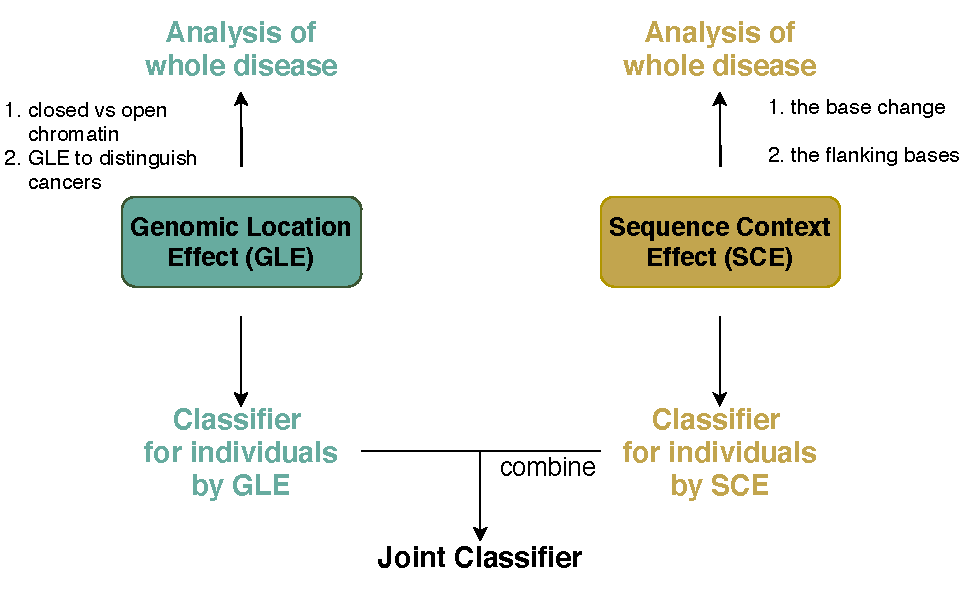
\includegraphics[scale=0.85]{graphics/workflow.pdf}
\caption{}
    % \caption{\textbf{Project workflow for understanding cancer mutagenesis data and exploiting it for cancer classification.} On one hand, cancers were analysed on the whole disease scale, which considered mutations from all donors of the same diseases as a whole. This magnified the signals in the data and made it easier for understanding the mutagenesis process. On the other hand, the information from the factors analysed above was used for training a classifier on the individual donor scale, meaning that this classifier could potentially be applied to a new patient's mutation data to predict their cancer. This followed a standard machine learning training procedure, outlined in Section \ref{methods:ml}.}
    \label{fig:workflow}
\end{figure}


\section{Data description}
\subsection{PCAWG - Mutation data:} 
The critical source of data for the project is the Pan-Cancer Analysis of Whole Genome (PCAWG) project \citep{Campbell2020}. This data consists of whole genome sequencing of both cancerous and healthy tissues (mostly blood) for all cancer patients. PCAWG relies on contrasting the cancerous against healthy tissues to determine whether a mutation is a \gls{sommut}. Identifying mutations by combining three established pipelines (Sanger \citep{Jones2016CgpCaVEManWrapper:Data}, EMBL/DKFZ \citep{Rimmer2014IntegratingApplications}, and Broad \citep{Cibulskis2013SensitiveSamples}), the project provides a valuable resource, which covers 2658 cancer samples from 28 cancer types, for studying cancer mutagenesis.

This project is limited to somatic \glspl{point_mut}. I sampled 12 cancers whose DHS data for the putative original cells is also available (Table \ref{tab:encode}). A summary of the mutations for the 12 cancers can be found in the appendix Table \ref{tab:mutation_summary} and Figure \ref{fig:mutation_summary}. Mutation data for all individuals and all mutations was downloaded as a MAF file from the \href{https://dcc.icgc.org/releases/PCAWG/consensus_snv_indel}{International Cancer Genome Consortium (ICGC)}. Driver mutations were then filtered out based on \href{https://dcc.icgc.org/releases/PCAWG/driver_mutations}{the PCAWG's driver mutation project} because driver mutations are under selection pressure and have different mutation rates to passenger mutations. The information this project utilised from PCAWG was the mutations, their genomic locations, their donor ID and the donor's cancer. 

\subsection{Reference genome:} 
To reconstruct the cancer genome, both mutation data and a standard human reference genome are required. The human reference genome was provided by Ensembl \citep{Yates2020Ensembl2020}, and downloaded from the \href{http://hgdownload.soe.ucsc.edu/goldenPath/hg19/chromosomes}{UCSC genome browser}. As PCAWG used Human Genome Assembly 37, the same version of genomic coordinates is used for this project. As an additional check, I also assert that the wildtype base at each mutated position and its local reference sequence context provided by PCAWG match the sequence at that position from the reference genome. 

\subsection{Chromatin status data:} 
Part of my project investigates the relationship between mutation distribution and chromatin status. Based on literature search, I identified the most likely tissue of origin for the cancer of interest, summarised in Table \ref{tab:encode}. DNase I hypersensitivity (DHS) data for these tissues of origin, as a canonical measure for chromatin status, was provided by ENCODE \citep[downloaded from either \href{https://genome.ucsc.edu/cgi-bin/hgFileUi?db=hg19&g=wgEncodeOpenChromDnase}{Duke} or \href{https://genome.ucsc.edu/cgi-bin/hgFileUi?db=hg19&g=wgEncodeUwDnase}{UW};][]{Thurman2012TheGenome,Klemm2019ChromatinEpigenome}. Specifically, ENCODE measured the level of Dnase hypersensitivity across the genome and identified Dnase hypersensitive regions based on an established threshold. Here, open chromatin regions are defined as the Dnase hypersensitive range and closed chromatin regions are the rest of the genome. The relationship between the original cells based on DHS can be visualised in Figure \ref{fig:encode_pca} via the multiple dimension scaling technique (details in Subsection \ref{methods:encode_pca}). 

\section{Algorithm development}
\subsection{Reproducibility} 
\href{http://git-scm.com}{Git} was used as a Version Control tool. Accordingly, the entire code history has been recorded and stored on \href{https://github.com}{GitHub}.

The entire project was done in loops, which means that most analyses were repeated on increasing scales. This not only increases the opportunity for code efficiency to be improved but also helps ensure that the algorithms are reproducible. 

While the project is too large to be shared in a thesis, all code is available upon request. 

\subsection{Developing packages}
Most core functions were written in Python \citep{van1995python}, with visualisation and some analyses written in R \citep{r}. Code was written as packages that can be installed and utilised by anyone with the permission. 

All core functions were tested under explicit hypothetical scenarios for correctness before being applied. This process is called unit testing. Each of the analyses requires multiple core functions. For each analysis, core functions are combined in one \href{https://click.palletsprojects.com/en/8.0.x/}{click} command that can be run either in the command line or conventional Python platforms such as Jupyter Notebook. The \href{https://github.com/HuttleyLab/scitrack}{Scitrack} Python package was applied to these commands so that not only code, but inputs and outputs of these commands were tracked as well.

\subsection{Parallelisation}
When analysing large data sets, some steps could be considerably time-consuming, particularly the initial data filtering step and the simulation steps. Therefore, for several steps, I have written scripts that optimise code parallelisation based on the original command line. By doing this, for an analysis that executes the same processes multiple times on independent objects, these objects were ``distributed'' into different computer cores instead of being processed sequentially on one single computer. This was supported by the National Computational Infrastructure Australia.


\section{Whole disease analysis of GLE}

The variation in chromatin structures of different cell types is believed to shape where mutations occur in the genome, giving rise certain patterns of GLE that are characteristic of cancers. The methods in this section serve two purposes: to formally test the presumed biological connection between chromatin structure and mutation locations, and to weigh the importance of GLE as a characteristic of the mutation profile irrespective of the its driving mechanism.  

\subsection{Visualising DHS by multi-dimensional scaling}\label{methods:encode_pca}
Before establishing the relationship between mutation location and chromatin structure, I examined whether and how the relevant original cells are related in terms of chromatin structure using DHS data. The rationale is that if chromatin structure is a true determinant of mutation location, then tissues that are epigenetically similar should have roughly similar patterns of GLE. Accordingly, this might partly explain the pattern of mis-classification by GLE afterwards.

For each pair of cell types, the intersections of their open chromatin regions were identified. The difference between the pair was then calculated as:

\begin{equation}
    d = 1 - \frac{2i}{o_1 + o_2}
\end{equation}

where $d$ is the difference/distance, $i$ is the total lengths of the genomic regions covered by the intersections, $o_1$ and $o_2$ are the length of the open chromatin regions. Essentially $d$ is the ``complement'' of the ratio between the intersection $i$ and the average length of the open regions $o_1$ and $o_2$. 

Once the distances for all possible pairs of cell types were obtained, I decomposed these distances into their relative coordinates by multi-dimensional scaling. This was done by the R function \texttt{cmdscale}. I reported the coordinates for the three most informative dimensions. %in the appendix?

\subsection{Mutation location in relation to chromatin status}
To establish the relationship between the mutation location of a cancer and the chromatin status of its original cell type, I sorted mutations into open and closed chromatin regions as per Figure \ref{fig:gle_workflow}. I then used 1. the G-test for whether we could reject the null that mutations occur without any preference for closed or open regions and 2. the odds ratio statistic to measure the bias towards closed regions.

\begin{figure}[h!]
    \centering
    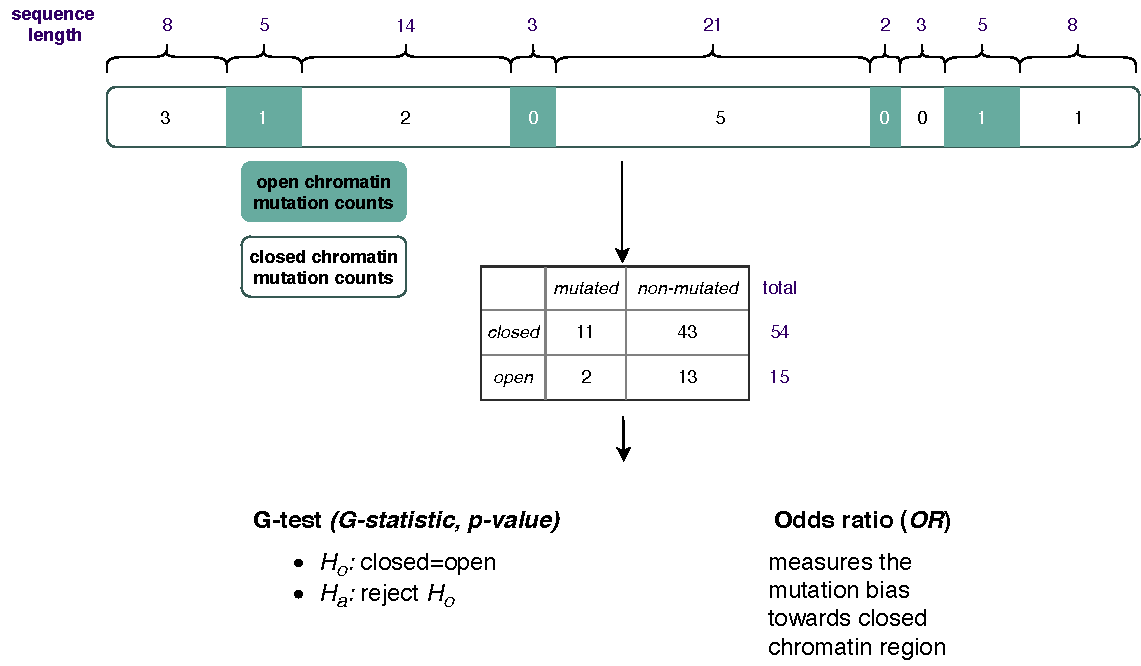
\includegraphics[scale=0.82]{graphics/mutdistribution.pdf}
\caption{}
    % \caption{\textbf{Establishing the relationship between cancer mutation and chromatin structure of the original cell type.} Mutations were sorted into open and closed regions to make a contingency table, from which a G-test can be performed and an Odds-ratio ($OR$) statistic can be calculated. The G-test establishes whether there is a significant bias in mutation location; $OR$ measures the degree of bias towards closed chromatin regions.}
    \label{fig:gle_workflow}
\end{figure}


\subsubsection{Homogeneity test for mutation location between closed and open regions}
I used the G-test of independence \citep{McDonald2014GtestStatistics} to examine the hypothesis whether the distribution of mutations are random across the genome - if this is the case, the expected number of mutations in the closed chromatin regions should not differ from that in the open regions. More formally:

\begin{itemize}
    \item $H_o (Null)$: Mutation abundance is independent of the chromatin status
    \item $H_a (Alternate)$: Mutation abundance is biased by the chromatin status
\end{itemize}

First, the expected number of observations for each cell was calculated as per Table \ref{tab:count_exp_demo}. For example, the expected number of mutated bases in the closed regions $e_i$ should be proportional to the number of bases available in the closed regions $c$ the number of mutations $m$. The departure of the observed count $o_i$ from the expected $e_i$ was measured by the $G$ statistic, calculated as:
\begin{equation}
    G = 2 \underset{i}{\sum} o_{i} \ln \frac{o_{i}}{e_{i}}
    \label{eq:g}
\end{equation}
where $o_{i}$ are observed values (\textit{i.e.} entries from Table \ref{tab:count_obs_demo}) and $e_{i}$ are expected values (\textit{i.e.} entries from Table \ref{tab:count_obs_demo}) and the p-value was obtained by permutation.

\vspace{0.2cm}
\begin{table}[ht!]
\caption{}
    % \caption{Demo contingency tables. Panel (a) contains the observed counts, each of the entries $c_m$, $c_n$, $o_m$ and $o_n$ represents an $o_i$ in equation \ref{eq:g}. Panel (b) contains the expected counts, each of the elements represents an $e_i$ in equation \ref{eq:g}.}
    \begin{subtable}[!h]{.5\textwidth}
        \centering
        \begin{tabular}{r|rr|r}
             & Mutated & Non-mutated & Total  \\
        \hline
            Closed & $c_m$ & $c_n$ & $c$ \\
            Open & $o_m$ & $o_n$ & $o$ \\
        \hline    
             & $m$ & $n$ & $t$ \\
        \end{tabular}
        \vspace{0.2cm}
    \subcaption{Observed counts}
    \label{tab:count_obs_demo}
    \end{subtable} 
    \quad % for side by side tables
    \begin{subtable}[!h]{.5\textwidth}
        \centering
        \begin{tabular}{r|rr|r}
             & Mutated & Non-mutated & Total  \\
        \hline     
            Closed & $c*m/t$ & $c*n/t$ & $c$ \\
            Open & $o*m/t$ & $o*n/t$ & $o$ \\
        \hline    
             & $m$ & $n$ & $t$ \\
        \end{tabular}
        \vspace{0.2cm}
    \subcaption{Expected counts}
    \label{tab:count_exp_demo}
    \end{subtable}    
\end{table}

\subsubsection{Odds ratio}
To complement the G-test, I used the odds ratio \citep[$OR$;][]{Hoppe2017OddsRatios} as a measure of preference for mutations to occur in closed chromatin regions compared to open regions. The formula for $OR$ of the contingency Table \ref{tab:count_obs_demo} is as follows:

\begin{equation}
    OR = \frac{c_m/c_n}{o_m/o_n}
    \label{eq:or}
\end{equation}

where $c_m$, $c_n$, $o_m$ and $o_n$ are all observed values that comes from Table \ref{tab:count_obs_demo}.
\subsubsection{Jackknife}
It is worth noting that even within one cancer type, different donors might vary in the number of mutations they carry and the locations of the mutations. If a donor has a very distinctive mutation pattern, then it is probable that the $OR$ statistic for their whole cancer cohort mostly represents that donor only. To address this, I performed a jackknife analysis on this measure for each disease \citep{Miller1974TheReview}. An illustration of the jackknife workflow is shown in figure \ref{fig:jackknife_demo}. Specifically, to see how influential a donor is on the $OR$, one simply removes that donor and observes how $OR$ changes. If one applies that to every donor, one obtains a new set of $OR$ that reflects the potential range of the true $OR$.



\subsubsection{Switching cell types}

\subsection{Hypothesis testing of GLE between cancer pairs by bootstrap}

\section{Whole disease analysis of SCE}
\section{Mutation-based classifier for cancers}
\subsection{Standard procedure}
\label{methods:ml}
\subsection{Combining GLE with SCE in a joint model}
